% Figure 1 -- Verifier in the loop (P3). English version.
% -------------------------------------------------------------------------
% GENERADO POR _figura_p3.py DEL REPOSITORIO MIGRA-IA. NO EDITAR A MANO:
% cualquier cambio se pierde al regenerar. Los numeros salen de
% data/figura_p3_verificador.csv; para llenar la figura se completa ese CSV
% y se vuelve a ejecutar el script.
%
% PAQUETES NECESARIOS EN EL PREAMBULO DEL .tex PRINCIPAL:
%   \usepackage{tikz}          ya esta (circulos Harvey de la Tabla I)
%   \usepackage{pgfplots}      NUEVO
%   \pgfplotsset{compat=1.18}  NUEVO
% Si falta alguno, la figura NO compila.
%
% ESTADO: MODO DISENO: el CSV no tiene ninguna medida todavia.
% -------------------------------------------------------------------------
\begin{figure}[t]
\centering
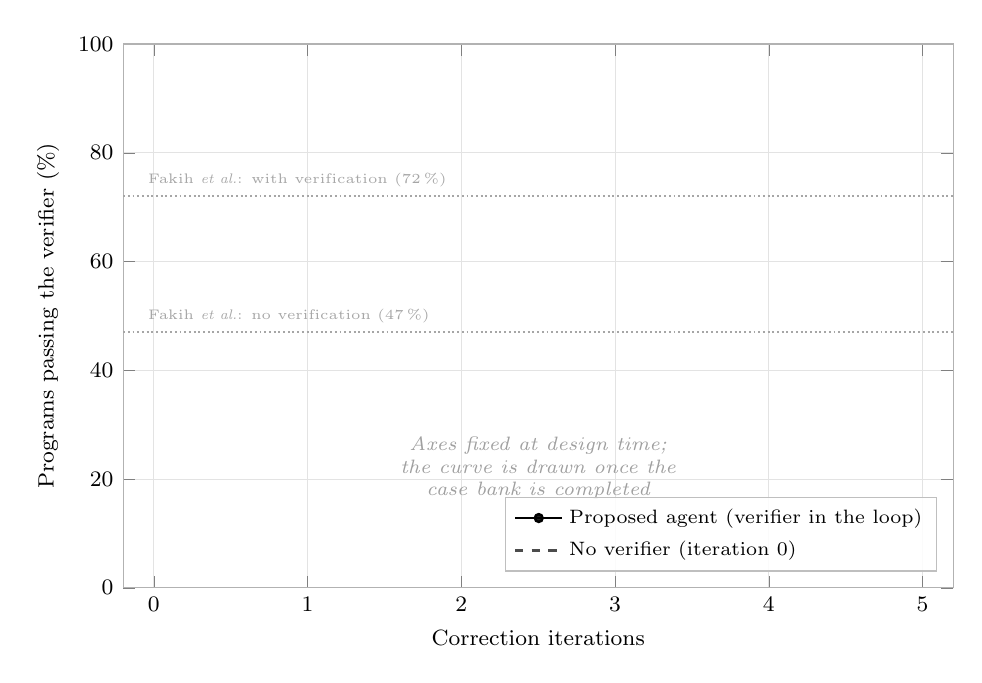
\begin{tikzpicture}
\begin{axis}[
  width=\columnwidth,
  height=0.70\columnwidth,
  xlabel={Correction iterations},
  ylabel={Programs passing the verifier (\%)},
  xmin=-0.2, xmax=5.2,
  ymin=0, ymax=100,
  xtick={0,1,2,3,4,5},
  ytick={0,20,40,60,80,100},
  grid=major,
  grid style={gray!22, line width=0.3pt},
  axis line style={gray!60},
  tick label style={font=\footnotesize},
  label style={font=\footnotesize},
  legend style={font=\scriptsize, at={(0.98,0.03)}, anchor=south east,
                draw=gray!50, fill=white, fill opacity=0.88, text opacity=1,
                row sep=1pt},
  legend cell align=left,
]

% --- Referencias externas publicadas (no son resultados de este trabajo) ---
\addplot[densely dotted, gray!70, line width=0.7pt, forget plot]
  coordinates {(-0.2,72.0) (5.2,72.0)};
\addplot[densely dotted, gray!70, line width=0.7pt, forget plot]
  coordinates {(-0.2,47.0) (5.2,47.0)};
\node[anchor=west, font=\tiny, text=gray!70] at (axis cs:-0.1,75.0)
  {Fakih \emph{et al.}: with verification (72\,\%)};
\node[anchor=west, font=\tiny, text=gray!70] at (axis cs:-0.1,50.0)
  {Fakih \emph{et al.}: no verification (47\,\%)};

% --- Curva propia: PENDIENTE. No se dibuja nada inventado. ---------------
\node[align=center, font=\scriptsize\itshape, text=gray!75]
  at (axis cs:2.5,22) {Axes fixed at design time;\\the curve is drawn once the\\case bank is completed};
\addlegendimage{black, mark=*, mark size=1.4pt, line width=0.9pt}
\addlegendentry{Proposed agent (verifier in the loop)}
\addlegendimage{dashed, black!70, line width=0.8pt}
\addlegendentry{No verifier (iteration 0)}

\end{axis}
\end{tikzpicture}
\caption{Share of generated programs that pass the verifier as a function of the number of correction iterations (subproblem P3). The reference line is generation without a verifier, that is, the value at iteration zero. Dotted lines reproduce the values reported by Fakih \emph{et al.} \cite{fakih2024llm4plc}, which are not results of this work. Axes and reference lines are fixed at design time; the curve is drawn once the case bank has been executed.}
\label{fig:verificador}
\end{figure}
